\documentclass[10pt]{article}
\usepackage{ctex}
\usepackage{CJK}
\usepackage{graphicx}
\usepackage{graphicx}
\bibliographystyle{plain}
\setlength{\parindent}{2em}
\begin{document}
\title{Stochastic resonance}
\author{Qilei Zhang}
\date{may 17 2018}
\maketitle
\par
\begin{figure}[htbp]
\small
\centering
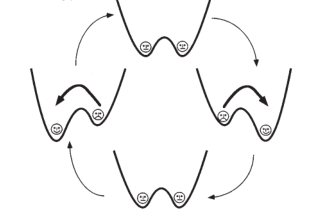
\includegraphics[width=20em]{000.png}
\caption{Figure:Stochastic resonance}
\label{fig:lable}
\end{figure}
\par
\section{background}
Over the last two decades, stochastic resonance has continuously attracted considerable attention. The term is given to a phenomenon that is manifest in nonlinear systems whereby generally feeble input information (such as a weak signal) can be be amplified and optimized by the assistance of noise.\cite{higham1994bibtex}
\par
\section{text}
The nonlinear system can increase the signal-to-noise ratio by optimizing the noise intensity. This phenomenon is called stochastic resonance. Stochastic resonance exists in the bistable system. Stochastic resonance is the phenomenon that under the certain nonlinear conditions, the output of the nonlinear system is enhanced by periodic output due to weak periodic signal and noise.\cite{h1994bibtex}
\par
Stochastic resonance was first proposed when studying the paleo-meteorological glaciers of the Earth. In the ancient times, the earth appeared alternately in the late heating period and the ice age. The sun exerts a cyclical effect on the Earth. However, this signal is weak and does not change the Earth's climate itself. Because the Earth is a nonlinear system, it generates a stochastic resonance phenomenon.
\par
\bibliography{aaa}
\footnote{\centering Stochastic resonance}
\end{document}

